% !TEX program = xelatex
% arXiv-style preprint · XeLaTeX + xeCJK
\documentclass[10pt,a4paper]{article}

% ── arXiv / preprint layout ──────────────────────────────────────────
\usepackage[margin=2.5cm]{geometry}
\usepackage{setspace}
\setstretch{1.15}

% ── Fonts (XeLaTeX) ─────────────────────────────────────────────────
\usepackage{fontspec}
\usepackage{xeCJK}
\setCJKmainfont{Source Han Serif CN}
\setCJKsansfont{Source Han Sans CN}
\setCJKmonofont{Source Han Sans CN}
\setmainfont{TeX Gyre Termes}[
  BoldFont={TeX Gyre Termes Bold},
  ItalicFont={TeX Gyre Termes Italic},
]
\setmonofont{Noto Sans Mono}

% ── Math & graphics ─────────────────────────────────────────────────
\usepackage{amsmath,amssymb,amsthm}
\usepackage{graphicx}
\usepackage{booktabs}
\usepackage{multirow}
\usepackage{array}
\usepackage{tikz}
\usetikzlibrary{arrows.meta,positioning,shapes.geometric,fit,calc}
\usepackage{pgfplots}
\pgfplotsset{compat=1.18}

% ── Code listing ────────────────────────────────────────────────────
\usepackage{listings}
\usepackage{xcolor}
\definecolor{codebg}{RGB}{248,248,242}
\definecolor{codekw}{RGB}{0.20,0.35,0.75}
\definecolor{codestr}{RGB}{0.72,0.20,0.20}
\definecolor{codecom}{RGB}{0.45,0.55,0.45}
\definecolor{codenum}{RGB}{0.40,0.25,0.55}
\lstdefinestyle{mailang}{
  backgroundcolor=\color{codebg},
  basicstyle=\ttfamily\small,
  keywordstyle=\color{codekw}\bfseries,
  stringstyle=\color{codestr},
  commentstyle=\color{codecom}\itshape,
  numberstyle=\tiny\color{gray},
  numbers=left,
  numbersep=6pt,
  frame=single,
  framerule=0.4pt,
  rulecolor=\color{gray!40},
  breaklines=true,
  showstringspaces=false,
  tabsize=4,
  columns=flexible,
  keepspaces=true,
  xleftmargin=1.6em,
  framexleftmargin=1.2em,
  morekeywords={fn,let,var,const,class,extends,trait,implements,override,return,
                if,elif,else,while,for,in,match,import,from,this,super,true,false,null},
}
\lstset{style=mailang}

% ── Hyperlinks / PDF ────────────────────────────────────────────────
\usepackage{hyperref}
\hypersetup{
  colorlinks=true,
  linkcolor=blue!50!black,
  citecolor=blue!50!black,
  urlcolor=blue!60!black,
  pdftitle={MaìLang: A Rust-Implemented Programming Language for IoT and Cross-Platform Development},
  pdfauthor={Maicarons},
}

% ── Theorem-like ────────────────────────────────────────────────────
\newtheorem{definition}{定义}
\newtheorem{design}{设计原则}

% ── Title block (arXiv preprint style) ──────────────────────────────
\title{%
  \textbf{MaìLang：面向物联网与跨平台开发的\\
  Rust 实现编程语言}\\[6pt]
  \large MaìLang: A Rust-Implemented Programming Language for\\
  IoT and Cross-Platform Development
}

\author{%
  Maicarons\\
  \texttt{https://github.com/Maicarons/mailang}
}

\date{%
  预印本（Preprint）\\
  版本 0.3.0 \quad · \quad 2026
}

\begin{document}

\maketitle

% ══════════════════════════════════════════════════════════════════
\begin{abstract}
物联网（IoT）与跨平台软件开发对编程语言提出了相互拉扯的需求：一方面需要足够小的运行时足迹与可预测的性能以适配 MCU 级设备，另一方面又需要现代语言特性（面向对象、模式匹配、错误处理、泛型）与多宿主嵌入能力。本文提出并实现 \textbf{MaìLang（麦语）}——一门以 Rust 编写、面向 IoT 与跨平台场景的现代编程语言。MaìLang 采用经典流水线架构（词法分析 $\rightarrow$ 语法分析 $\rightarrow$ 字节码编译 $\rightarrow$ 虚拟机），默认后端为带槽位局部变量（slot locals）的栈式字节码虚拟机，并提供特性对齐的可选寄存器虚拟机。语言层面融合了类与继承、Trait、Rust 风格的 \texttt{Result}/\texttt{Option} 与 \texttt{?} 错误传播、模式匹配、字符串插值、UTF-8 原生标识符以及泛型函数 monomorphization；运行时层面实现了引用计数、环收集与标记清扫堆的混合垃圾回收，以及 \texttt{CallDirect}、尾调用优化（TCO）等热路径优化。跨平台能力通过 C FFI、WebAssembly、模拟 HAL 与多语言绑定演示覆盖 12 种宿主语言。实验表明：在 Fibonacci(30) 递归基准上，优化后的 MaìLang 约需 137\,ms，相对早期基线加速约 $4.25\times$；在循环、函数调用与字符串插值等典型负载上优于 CPython 与 Node.js（V8）。集成测试套件在栈式与寄存器两种虚拟机上均达 102/102 通过率，全工作区约 218 项测试全绿。本文系统描述 MaìLang 的语言设计、编译器与虚拟机实现、内存管理策略与跨平台嵌入方案，并诚实报告当前局限（无 \texttt{async}、泛型类字段擦除、IoT HAL 默认模拟等）。
\end{abstract}

\vspace{1em}
\noindent\textbf{关键词：} 编程语言实现；物联网；字节码虚拟机；Rust；跨平台嵌入；垃圾回收；monomorphization

% ══════════════════════════════════════════════════════════════════
\section{引言}
\label{sec:intro}

物联网（Internet of Things, IoT）设备与跨平台应用构成了当代系统软件的两大增长极。从运行在 ESP32-C3、Cortex-M4 等 MCU 上的传感器固件，到需要在浏览器、桌面与移动端共享逻辑的业务应用，开发者反复面临同一组张力：\emph{资源受限环境要求的精简运行时}与\emph{现代应用开发要求的表达能力}往往难以兼得。

现有方案各有取舍。C/C++ 与 Rust 提供极致性能与小足迹，但学习曲线陡峭、开发迭代慢；Python 与 JavaScript 生态丰富，但解释器体积与内存占用对 MCU 不友好；Lua 与 MicroPython 面向嵌入做了裁剪，却在类型表达、错误处理与工具链完整性上偏弱；WebAssembly 解决了分发问题，但其本身并不提供高级语言特性。换言之，\textbf{尚缺一门同时覆盖「现代语言特性 + 可控足迹 + 多宿主嵌入」的实用语言}。

MaìLang（麦语）正是针对这一缺口的设计与实现。文件扩展名为 \texttt{.mai}，实现语言为 Rust，核心目标包括：

\begin{enumerate}
  \item \textbf{现代语言特性}：类与继承、Trait、闭包、模式匹配、\texttt{Result}/\texttt{Option} 与 \texttt{?}、字符串插值、UTF-8 标识符、泛型函数 monomorphization。
  \item \textbf{可预测的解释执行}：默认栈式字节码虚拟机（slot locals + \texttt{CallDirect} + TCO），可选寄存器虚拟机实现特性对齐。
  \item \textbf{混合内存管理}：\texttt{Rc} 引用计数 + \texttt{collect\_cycles()} 断环 + 标记清扫堆（\texttt{MarkSweepHeap}）。
  \item \textbf{跨平台嵌入}：C ABI FFI、WebAssembly、模拟 HAL、多语言绑定，以及字节码产物 \texttt{.mailangbc}。
  \item \textbf{工程完备性}：解析器错误恢复、分析器、LSP、格式化器、模块系统 v2、文件/静态 HTTP 包注册表。
\end{enumerate}

本文贡献如下：

\begin{itemize}
  \item 提出并实现 MaìLang 语言设计与完整实现流水线，全部以 Rust 工作区组织为 16 个 crate，覆盖词法、语法、分析、编译、虚拟机、GC、标准库、FFI、WASM、LSP 与包管理。
  \item 给出栈式/寄存器双后端的字节码虚拟机设计，并在两种后端上通过同一套 102 项集成测试验证特性对齐。
  \item 实现面向 IoT 场景的混合 GC（引用计数 + 环断边 + 标记清扫）与一系列热路径优化（胖 \texttt{Value} 的 \texttt{Rc} 化、全局槽表、立即数融合、\texttt{CallDirect} 等），使 Fibonacci(30) 相对早期基线加速约 $4.25\times$。
  \item 提供覆盖 C、Python、Node.js、Go、Java、Kotlin、C\#、Swift、PHP、Ruby、Lua、TypeScript 共 12 种宿主的绑定演示与可复现基准，并诚实报告局限。
\end{itemize}

% ══════════════════════════════════════════════════════════════════
\section{相关工作}
\label{sec:related}

\paragraph{嵌入式脚本语言。}
Lua 是嵌入式脚本的经典范例，以极小运行时与 C API 友好著称\cite{lua}，但其动态类型系统与弱错误处理模型难以支撑大型应用。MicroPython 将 Python 语义裁剪到 MCU，极大地降低了嵌入开发门槛\cite{micropython}，却同样受制于动态语义带来的隐式错误与有限的静态检查。QuickJS 是一款紧凑的 JavaScript 解释器，采用寄存器式字节码，在解释器性能上表现优异\cite{quickjs}，但宿主被限定在 ECMAScript 语义内。

\paragraph{系统语言与安全运行时。}
Rust 以所有权与生命周期在系统层兼顾安全与性能\cite{rust}，是实现语言工具链的常见选择；MaìLang 将 Rust 用作\emph{实现语言}，而非目标语言。Java 与 C\# 证明了带 GC 的托管运行时在工业界的可行性\cite{java,csharp}，但其运行时体积与启动成本对 MCU 场景并不友好。

\paragraph{WebAssembly 与跨语言嵌入。}
WebAssembly 提供了可移植、沙箱化的分发格式\cite{wasm}，适合作为跨平台目标之一，但不替代语言前端与运行时语义。通过 C ABI 导出宿主函数注册接口是跨语言嵌入的稳妥路径\cite{ffi}，MaìLang 的 FFI 层即采用此设计，并由 \texttt{cbindgen} 自动生成头文件。

\paragraph{编译器与虚拟机技术。}
栈式虚拟机实现简单、字节码紧凑，是教学与嵌入场景的常见选择；寄存器式虚拟机减少指令分派次数，在热点负载上更有优势\cite{vm-design}。monomorphization 是 C++/Rust 实现零成本泛型的主流手段\cite{generics}；MaìLang 将其用于泛型函数，并对泛型类采用字段擦除以控制实现复杂度。垃圾回收方面，引用计数无法单独处理环结构，通常需辅以环收集或追踪式回收\cite{gc}——MaìLang 的混合方案正对应这一观察。

与上述工作相比，MaìLang 的定位是：\textbf{以现代静态风格语法组织 IoT/跨平台应用逻辑，以字节码解释器保证足迹可控，以 FFI/WASM/HAL 覆盖多宿主}，并提供完整的语言工具链与包管理闭环。

% ══════════════════════════════════════════════════════════════════
\section{语言设计}
\label{sec:language}

\subsection{概览与语法}

MaìLang 源文件扩展名为 \texttt{.mai}。代码~\ref{lst:hello} 展示了基本语法：函数、类型标注、字符串插值与 UTF-8 标识符。

\begin{lstlisting}[language={},caption={MaìLang 基本语法示例},label={lst:hello},float]
// hello.mai
fn greet(name: str) -> str {
    return "你好，{name}！"
}

println(greet("MaiLang"))
\end{lstlisting}

\begin{definition}[MaìLang 程序]
一个 MaìLang 程序是若干语句（\texttt{Stmt}）构成的序列，经词法分析得到 \texttt{Token} 流，由递归下降 + Pratt 解析器构造抽象语法树（\texttt{Program}/\texttt{Stmt}/\texttt{Expr}/\texttt{Pattern}），再编译为分块字节码（\texttt{Chunk}/\texttt{Bytecode}）供虚拟机执行。
\end{definition}

\subsection{变量、函数与控制流}

变量通过 \texttt{let}（不可变）、\texttt{var}（可变）与 \texttt{const}（常量）声明，编译器强制可变性——对 \texttt{let}/\texttt{const} 赋值将在语义分析阶段被拒绝。函数支持默认参数、递归、闭包捕获与尾调用优化。控制流包含 \texttt{if}/\texttt{elif}/\texttt{else}、\texttt{while}、\texttt{for}\,$\in$\,range 与后缀 \texttt{expr match \{ \}}。

\subsection{面向对象与 Trait}

MaìLang 支持类、单继承、构造函数（\texttt{init}）、\texttt{super()} 调用、\texttt{super.method()} 以及 \texttt{override}。Trait 通过 \texttt{implements} 挂到类上，支持默认方法与 \texttt{trait extends}（trait 继承）。代码~\ref{lst:oop} 给出示意。

\begin{lstlisting}[language={},caption={类继承与 Trait},label={lst:oop},float]
class Animal {
    let name: str
    fn init(name: str) { this.name = name }
    fn speak() -> str { return "{this.name} speaks" }
}

class Dog extends Animal {
    override fn speak() -> str {
        return "{this.name} barks!"
    }
}

trait Printable {
    fn to_string() -> str
    fn print() { println(this.to_string()) }
}
\end{lstlisting}

\subsection{模式匹配与错误处理}

模式匹配支持字面量、区间、\texttt{Ok}/\texttt{Err}/\texttt{Some}/\texttt{None}、或模式、守卫，以及数组/元组解构。错误处理采用 Rust 风格的 \texttt{Result<T,E>} / \texttt{Option<T>} 与 \texttt{?} 传播算子，见代码~\ref{lst:match}。

\begin{lstlisting}[language={},caption={模式匹配与 Result/Option},label={lst:match},float]
fn classify(n) {
    match n {
        0 => "zero"
        1..10 => "small"
        _ => "other"
    }
}

fn divide(a: float, b: float) -> Result<float, str> {
    if b == 0.0 { return Err("Division by zero") }
    return Ok(a / b)
}
\end{lstlisting}

\subsection{泛型}

泛型函数采用 monomorphization：turbofish 语法 \texttt{id::<int>(x)} 将调用点特化为独立 chunk（命名 \texttt{id\$int}），从而避免运行时类型擦除开销。泛型类目前采用字段擦除布局（单布局、字段动态），不进行按类型布局特化——这是有意的实现取舍，见第~\ref{sec:limits} 节。

\subsection{模块与包}

模块系统 v2 采用「文件即模块」模型，\texttt{mailang.toml} 声明路径依赖（\texttt{mailang deps} 解析）。包注册表支持文件系统目录与静态 HTTP 镜像，提供 \texttt{publish}/\texttt{install}/\texttt{search}/\texttt{yank} 子命令。该设计刻意避免对中心化托管服务的依赖，以适配离线/内网 IoT 开发场景。

% ══════════════════════════════════════════════════════════════════
\section{系统架构与实现}
\label{sec:arch}

\subsection{总体流水线}

MaìLang 遵循经典编译器流水线，全部组件以 Rust crate 形式组织：

\begin{equation*}
  \text{Source (.mai)}
  \;\xrightarrow{\text{Lexer}}\;
  \text{Tokens}
  \;\xrightarrow{\text{Parser}}\;
  \text{AST}
  \;\xrightarrow{\text{Compiler}}\;
  \text{Bytecode}
  \;\xrightarrow{\text{VM}}\;
  \text{Value}
\end{equation*}

图~\ref{fig:arch} 给出 crate 依赖与数据流。表~\ref{tab:crates} 汇总各 crate 职责。

\begin{figure}[t]
\centering
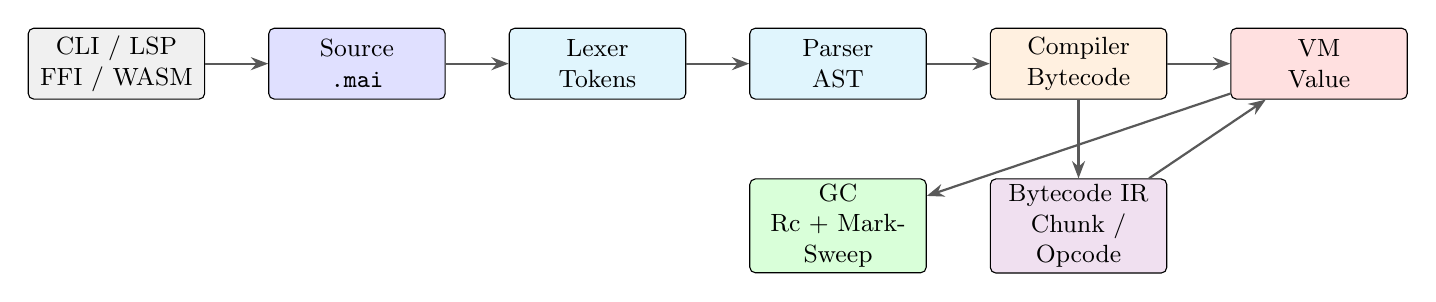
\begin{tikzpicture}[
  font=\small,
  boxbase/.style={draw, rounded corners=2pt, align=center,
              minimum height=9mm, minimum width=22mm,
              text width=21mm, inner sep=2pt},
  boxA/.style={boxbase, fill=blue!12},
  boxB/.style={boxbase, fill=cyan!12},
  boxC/.style={boxbase, fill=orange!12},
  boxD/.style={boxbase, fill=red!12},
  boxE/.style={boxbase, fill=green!15},
  boxF/.style={boxbase, fill=violet!12},
  boxG/.style={boxbase, fill=gray!12},
  arr/.style={-{Stealth[length=2.2mm]}, thick, gray!70!black},
]
\node[boxA]  (src)  {Source\\ \texttt{.mai}};
\node[boxB, right=8mm of src] (lex)  {Lexer\\ Tokens};
\node[boxB, right=8mm of lex]  (ast)  {Parser\\ AST};
\node[boxC, right=8mm of ast] (cmp) {Compiler\\ Bytecode};
\node[boxD, right=8mm of cmp]   (vm)   {VM\\ Value};

\draw[arr] (src) -- (lex);
\draw[arr] (lex) -- (ast);
\draw[arr] (ast) -- (cmp);
\draw[arr] (cmp) -- (vm);

\node[boxE, below=10mm of ast] (gc) {GC\\ Rc + Mark-Sweep};
\node[boxF, below=10mm of cmp] (bc) {Bytecode IR\\ Chunk / Opcode};
\draw[arr] (vm) -- (gc);
\draw[arr] (cmp) -- (bc);
\draw[arr] (bc) -- (vm);

\node[boxG, left=8mm of src] (cli) {CLI / LSP\\ FFI / WASM};
\draw[arr] (cli) -- (src);
\end{tikzpicture}
\caption{MaìLang 编译与执行流水线。上游为宿主集成层（CLI、LSP、FFI、WASM），下游为字节码 IR 与虚拟机，GC 跟踪运行时堆节点。}
\label{fig:arch}
\end{figure}

\begin{table}[t]
\centering
\caption{MaìLang Rust 工作区 crate 概览（共 16 个）。}
\label{tab:crates}
\small
\begin{tabular}{@{}llp{6.8cm}@{}}
\toprule
\textbf{Crate} & \textbf{阶段} & \textbf{职责} \\
\midrule
mailang-lexer & 词法 & Unicode 感知分词 \\
mailang-ast & 语法 & AST 数据结构（含 serde） \\
mailang-parser & 语法 & 递归下降 + Pratt；错误恢复 \\
mailang-analyzer & 语义 & 诊断 / 参数个数 / 简单类型 \\
mailang-compiler & 编译 & 字节码生成；泛型 monomorphization \\
mailang-bytecode & IR & 栈式 IR + 寄存器 IR；\texttt{Value} \\
mailang-vm & 执行 & 栈式 VM（默认）+ 寄存器 VM \\
mailang-gc & 内存 & 断环 + \texttt{MarkSweepHeap} \\
mailang-stdlib & 运行时 & io/math/string/json/time/HAL \\
mailang-core & 集成 & Parser $\rightarrow$ Compiler $\rightarrow$ VM \\
mailang-cli & 工具 & run/eval/build/fmt/deps/registry/lsp \\
mailang-ffi & 嵌入 & C ABI；host 函数注册 \\
mailang-wasm & 嵌入 & wasm-bindgen；\texttt{eval} / \texttt{eval\_json} \\
mailang-lsp & 工具 & 诊断/补全/跳转/悬停 \\
mailang-module & 包 & 模块 v2 + 路径依赖 + 注册表 \\
mailang-macros & 扩展 & 过程宏（当前为透传桩） \\
\bottomrule
\end{tabular}
\end{table}

\subsection{词法与语法分析}

词法分析器对 UTF-8 标识符原生支持，并接受十六进制/八进制/二进制字面量与块注释。语法分析器采用递归下降处理语句与声明、Pratt 处理表达式优先级；关键特性是\textbf{解析错误恢复}（\texttt{recover\_from\_error} / \texttt{parse\_program\_recovering}），使 LSP 能在一次诊断中报告多条语法错误，而非在首个错误处终止。

\subsection{字节码与编译器}

字节码以 \texttt{Chunk} 为单位组织：每个函数对应一个 chunk，拥有独立的指令列表与常量池，主代码为 chunk 0。全局变量通过常量池名称解析，局部变量在编译期解析为栈槽位（slot），闭包经 upvalue 捕获。图~\ref{fig:vm} 展示两种执行模型。

\begin{figure}[t]
\centering
\begin{tikzpicture}[
  font=\small,
  cell/.style={draw, minimum width=7mm, minimum height=6mm,
               fill=#1!25, inner sep=0pt},
  lbl/.style={font=\footnotesize},
]
% Stack VM
\node[lbl, anchor=west] at (0,1.6) {\textbf{(a) 栈式 VM + slot locals}};
\foreach \i/\c in {0/blue, 1/blue, 2/orange, 3/orange, 4/green, 5/green} {
  \node[cell=\c] (s\i) at ({0.35+\i*0.75}, 0.7) {};
}
\node[lbl] at (2.2,-0.15) {栈槽位 / 局部变量};
\node[draw, rounded corners=2pt, minimum width=28mm, minimum height=8mm,
      fill=red!10] at (7.2, 0.7) {PC $\rightarrow$ Opcode};
\draw[-{Stealth}, thick, gray] (5.0, 0.7) -- (5.7, 0.7);

% Register VM
\node[lbl, anchor=west] at (0,-2.2) {\textbf{(b) 寄存器 VM（可选后端）}};
\foreach \i/\c in {0/violet, 1/violet, 2/violet, 3/violet, 4/violet} {
  \node[cell=\c] (r\i) at ({0.35+\i*0.75}, -3.1) {R\i};
}
\node[draw, rounded corners=2pt, minimum width=32mm, minimum height=8mm,
      fill=red!10] at (7.2, -3.1) {RegOp：dst/src 寻址};
\draw[-{Stealth}, thick, gray] (4.2, -3.1) -- (5.5, -3.1);
\end{tikzpicture}
\caption{两种虚拟机后端：(a) 默认栈式虚拟机，局部变量解析为栈槽位；(b) 可选寄存器虚拟机，将栈操作降为 \texttt{RegOp} 的 dst/src 寄存器寻址。两后端通过同一套 102 项集成测试。}
\label{fig:vm}
\end{figure}

编译器在调用点区分两类函数调用：已知顶层函数且未被局部遮蔽时生成 \texttt{CallDirect}（跳过函数值占位槽），否则走通用 \texttt{Call}。对自递归尾调用复用栈帧实现 TCO。泛型函数在出现 turbofish 或唯一类型参数位置时触发 monomorphization，特化结果以 \texttt{name\$type} 命名缓存。

\subsection{虚拟机}

默认后端为带槽位局部变量的栈式虚拟机。运行时值 \texttt{Value} 是统一的动态类型枚举，覆盖 \texttt{Null}/\texttt{Bool}/\texttt{Int}/\texttt{Float}/\texttt{Str}/\texttt{Char}/\texttt{Array}/\texttt{Map}/\texttt{Tuple}/\texttt{Function}/\texttt{Closure}/\texttt{Class}/\texttt{Instance}/\texttt{Ok}/\texttt{Err}/\texttt{Some} 等变体。堆对象经 \texttt{Rc}/\texttt{Rc<RefCell<\dots>>} 共享，避免深拷贝。

可选寄存器虚拟机通过 \texttt{MAILANG\_VM=register} 或 \texttt{--vm=register} 启用，将栈 IR 降为寄存器 IR，与栈式后端保持特性对齐。

\subsection{内存管理}
\label{sec:gc}

单纯引用计数无法回收环结构（自引用实例、互相引用的数组等）。MaìLang 采用三层策略：

\begin{enumerate}
  \item \textbf{日常分配/释放}：\texttt{Rc} 引用计数，热路径零额外开销；
  \item \textbf{环断边}：\texttt{collect\_cycles()} 从根出发 DFS，在灰集中发现回边时将其替换为 \texttt{Null}，使环可被引用计数释放；
  \item \textbf{标记清扫}：\texttt{MarkSweepHeap} 维护堆节点普查表（heap census），从 VM 根（栈 / 全局 / upvalue）标记可达节点，清扫不可达节点并清除子边，从而真正回收环状垃圾。分配计数越过阈值时自动触发回收，阈值随回收次数增长（经典「代际提示」风格）。
\end{enumerate}

\texttt{gc\_stats()} 暴露（tracked, collections, freed）统计，便于嵌入宿主观察回收行为。增量/并发 GC 尚未实现，见第~\ref{sec:limits} 节。

\subsection{性能优化}
\label{sec:perf}

相对早期基线，MaìLang 实施了如下热路径优化：

\begin{itemize}
  \item 堆对象 \texttt{Value} 改为 \texttt{Rc} 共享，消除深拷贝；
  \item 全局变量改为 \texttt{Vec} 槽表，\texttt{Load/StoreGlobal} 免哈希与字符串克隆；
  \item 数组/字典写操作原地修改；
  \item 自递归尾调用复用栈帧（TCO）；
  \item \texttt{CallDirect} 调用已知顶层函数，去掉函数占位槽；
  \item 算术/跳转立即数融合；
  \item workspace release 采用 \texttt{lto} + \texttt{codegen-units=1} + \texttt{panic="abort"}。
\end{itemize}

\subsection{跨平台与嵌入}

\paragraph{C FFI。}
\texttt{mailang-ffi} 导出稳定 C ABI，支持宿主函数注册与全局读写；头文件由 \texttt{cbindgen} 依据 \texttt{cbindgen.toml} 自动生成。特性开关 \texttt{std}/\texttt{gc} 映射为 C 宏 \texttt{MAILANG\_STD}/\texttt{MAILANG\_GC}。

\paragraph{WebAssembly。}
\texttt{mailang-wasm} 经 wasm-bindgen 暴露 \texttt{eval} / \texttt{eval\_json}，可在浏览器与 Node 中运行，并配有在线 Playground。

\paragraph{IoT HAL。}
标准库提供 \texttt{gpio\_*}、\texttt{adc\_read}、\texttt{delay\_ms} 等硬件抽象接口。\textbf{默认实现为宿主模拟}；真实硬件需通过 FFI 注册 HAL。交叉编译目标覆盖 \texttt{wasm32-unknown-unknown}、\texttt{thumbv7em-none-eabihf}（Cortex-M4）与 \texttt{riscv32imc-unknown-none-elf}（ESP32-C3）。

\paragraph{多语言绑定。}
仓库提供 12 种宿主语言的绑定演示（C、C\#、Go、Java、Kotlin、Lua、Node.js、PHP、Python、Ruby、Swift、TypeScript），验证 C ABI 的通用性。

\subsection{工具链}

CLI 提供 \texttt{run}/\texttt{eval}/\texttt{build}/\texttt{fmt}/\texttt{deps}/\texttt{registry}/\texttt{lsp}；字节码可持久化为 \texttt{.mailangbc}。LSP 基于 parser 错误恢复，支持多语法错误诊断与补全、跳转、悬停。分析器提供参数个数与简单类型诊断。

% ══════════════════════════════════════════════════════════════════
\section{实验与评估}
\label{sec:eval}

\subsection{实验环境}

所有性能数据来自 Windows 11 桌面环境（Intel CPU），Rust stable 工具链，\texttt{cargo build --release} 构建；基准取 7 次运行平均值。对比解释器包括 CPython 3.14、Node.js（V8 JIT）与 QuickJS（2025-04-26）。MaìLang 为 0.3.0（Phase L，栈式字节码解释器 + slot locals）。

\subsection{正确性测试}

集成测试套件共 102 项，覆盖算术、变量可变性、函数与默认参数、闭包、控制流、字符串插值、集合方法、模式匹配、OOP 与 Trait、\texttt{Result}/\texttt{Option} 与 \texttt{?}、模块导入、GC 回收路径等。如表~\ref{tab:tests} 所示，\textbf{栈式与寄存器两种虚拟机后端均 102/102 通过}，全工作区约 218 项测试全绿，验证了双后端特性对齐。

\begin{table}[t]
\centering
\caption{集成测试通过率。}
\label{tab:tests}
\small
\begin{tabular}{@{}lcc@{}}
\toprule
\textbf{执行后端} & \textbf{通过 / 总数} & \textbf{说明} \\
\midrule
栈式 VM（默认） & 102/102 & \texttt{mailang run} \\
寄存器 VM（可选） & 102/102 & \texttt{MAILANG\_VM=register} \\
全工作区测试 & 约 218 全绿 & 含单元与集成 \\
\bottomrule
\end{tabular}
\end{table}

\subsection{性能结果}

\paragraph{递归热点：Fibonacci(30)。}
在完成 $F_1$--$F_5$ 热路径优化（Rc 胖 \texttt{Value}、热路径、立即数融合、\texttt{CallDirect} 无占位、\texttt{panic=abort}）后，Fibonacci(30) 递归（结果 832040）约需 \textbf{137\,ms}（含约 11\,ms 进程启动），相对 Phase A 基线 581.59\,ms 加速约 \textbf{$4.25\times$}，达到预定 $3\times$ 验收目标。图~\ref{fig:accel} 展示加速前后对比。

\begin{figure}[t]
\centering
\begin{tikzpicture}
\begin{axis}[
  ybar,
  bar width=18pt,
  width=0.72\textwidth,
  height=5.4cm,
  ylabel={时间（ms，越低越好）},
  symbolic x coords={Phase A 基线, Phase F 优化后},
  xtick=data,
  ymin=0,
  ymax=650,
  nodes near coords,
  every node near coord/.append style={font=\small, rotate=0},
  grid=major,
  grid style={dashed, gray!35},
]
\addplot[fill=blue!35] coordinates {(Phase A 基线, 581.59) (Phase F 优化后, 137.0)};
\end{axis}
\end{tikzpicture}
\caption{Fibonacci(30) 递归基准：Phase A 基线与 Phase F 优化后的耗时对比（release 构建，7 次平均）。加速比约 $4.25\times$。}
\label{fig:accel}
\end{figure}

\paragraph{与 Python / Node.js / QuickJS 的对比。}
表~\ref{tab:bench} 给出四项典型负载的横向对比（越低越好）。可以看出：MaìLang 在循环、函数调用与字符串插值上均快于 CPython 与 Node.js；相对同为解释器的 QuickJS，字符串插值基本持平，循环与调用仍有差距，深度递归差距最大——这与解释器缺少内联缓存、无寄存器分配有关，也是后续优化方向。

\begin{table}[t]
\centering
\caption{典型负载耗时对比（ms，7 次平均；越低越好）。QuickJS 列中「—」表示未测。}
\label{tab:bench}
\small
\begin{tabular}{@{}lrrrr@{}}
\toprule
\textbf{基准} & \textbf{MaìLang} & \textbf{CPython} & \textbf{Node.js} & \textbf{QuickJS} \\
\midrule
Fibonacci(30) 递归 & 581.6$^{\dagger}$ & 165.5 & — & 70.6 \\
循环 sum $0..100$k & 35.4 & 105.2 & 53.8 & 9.8 \\
函数调用 $100$k & 45.6 & 100.9 & 51.2 & 16.0 \\
字符串插值 $10$k & 9.2 & 91.2 & 47.8 & 9.2 \\
\midrule
Fibonacci(30)（优化后） & \textbf{137.0} & — & — & 70.6 \\
\bottomrule
\end{tabular}
\\[2pt]
{\footnotesize $^{\dagger}$ 为 Phase A 基线，对应表中与 Python/Node/QuickJS 同批测量；优化后数据为 Phase F 单独复测。}
\end{table}

\paragraph{相对优势的量化。}
以 Phase A 基线口径计算：循环负载较 CPython 快约 $3.0\times$、较 Node.js 快约 $1.5\times$；函数调用较 CPython 快约 $2.2\times$；字符串插值较 CPython 快约 $9.9\times$、较 Node.js 快约 $5.2\times$，与 QuickJS 持平。优化后 Fibonacci(30)（137\,ms）已接近 QuickJS（70.6\,ms）的 $1.94\times$ 范围，而仍具备 CPython 之外的现代语言特性集合。

\paragraph{IoT 场景推算。}
以 ESP32-C3 @ 160\,MHz 相对现代 PC 慢 $50$--$100\times$ 的经验系数外推：循环 $100$k 约 $1.8$--$3.5$\,s，字符串插值 $10$k 约 $0.5$--$0.9$\,s。相较 MicroPython 的经验估计，MaìLang 在循环与字符串密集负载上预计有 $2$--$10\times$ 优势。需要强调：该推算\textbf{尚未在真实硬件上验证}，当前 IoT HAL 为模拟实现。

\subsection{产物体积}

字节码以 \texttt{.mailangbc} 形式持久化，便于嵌入宿主免源码分发。编译目标在 CI 中对 \texttt{thumbv7em-none-eabihf} 与 \texttt{riscv32imc-unknown-none-elf} 做体积约束检查。详细足迹数据随发布流程持续补充。

% ══════════════════════════════════════════════════════════════════
\section{讨论与局限}
\label{sec:limits}

\paragraph{无 \texttt{async}。}
当前不提供 async/await 语法与运行时。对事件驱动的 IoT 固件，状态机式回调或协作式多任务是可接受的替代；对高并发服务端场景则构成明显短板。

\paragraph{泛型类字段擦除。}
泛型函数已完成 monomorphization，但泛型类采用单一擦除布局，字段保持动态。这限制了字段访问的静态优化空间，也使完整泛型类型检查无法落实。

\paragraph{IoT HAL 默认模拟。}
\texttt{gpio\_*} 等接口默认由宿主模拟，真实硬件需 FFI 注册。本文报告的 IoT 数字为推算，不构成真实硬件验证声明。

\paragraph{GC 非增量。}
Rc + 标记清扫可回收环，但回收过程非增量/并发，最坏延迟不可控。对硬实时 MCU 场景需进一步做分配预算或区域式内存策略。

\paragraph{寄存器 VM 为可选后端。}
尽管与栈式后端特性对齐（102/102），默认后端仍是栈式 VM；寄存器后端的长期维护成本需在路线图中评估。

\paragraph{注册表与宏。}
包注册表仅支持本地/静态 HTTP，无公共托管服务；\texttt{mailang-macros} 仍为透传桩，过程宏体系尚未落地。

% ══════════════════════════════════════════════════════════════════
\section{结论}
\label{sec:concl}

本文提出了 MaìLang（麦语）——一门以 Rust 实现、面向 IoT 与跨平台开发的现代编程语言。通过「现代语言特性 + 字节码解释执行 + 混合 GC + 多宿主嵌入」的组合设计，MaìLang 在表达能力与运行时可控性之间取得了务实平衡。双虚拟机后端通过同一套 102 项集成测试验证特性对齐；热路径优化使 Fibonacci(30) 相对早期基线加速约 $4.25\times$；在循环、函数调用与字符串插值等典型负载上优于 CPython 与 Node.js。

未来工作包括：真实 IoT HAL 与硬件验证、增量 GC、泛型类 monomorphization、\texttt{async} 支持、寄存器 VM 深度优化，以及公共包注册表服务。我们希望 MaìLang 能为「一门语言贯通 MCU 与云端」的工程实践提供可复用的参考实现。

% ══════════════════════════════════════════════════════════════════
\section*{致谢}

本项目以 Apache-2.0 许可证开源。感谢 Rust 社区提供的工程基础设施，以及所有在语言设计讨论中给出反馈的同行。

% ══════════════════════════════════════════════════════════════════
\begin{thebibliography}{20}

\bibitem{lua}
R. Ierusalimschy, L. H. de Figueiredo, and W. Celes,
``Lua --- an extensible extension language,''
\emph{Software: Practice and Experience}, vol.~26, no.~6, pp.~625--652, 1996.

\bibitem{micropython}
D. P. George and G. M. T. Group,
``MicroPython: Python for microcontrollers,''
\emph{GitHub / micropython project}, 2014.
\url{https://micropython.org}

\bibitem{quickjs}
F. Bellard,
``QuickJS: A small and embeddable JavaScript engine,''
2019. \url{https://bellard.org/quickjs/}

\bibitem{rust}
N. D. Matsakis and F. S. Klock,
``The Rust Programming Language,''
\emph{ACM SIGAda Ada Letters}, vol.~34, no.~3, pp.~103--104, 2014.

\bibitem{java}
J. Gosling, B. Joy, G. Steele, G. Bracha, and A. Buckley,
\emph{The Java Language Specification}, Java SE 21 ed.
Oracle, 2023.

\bibitem{csharp}
E. Meijer and M. Torgersen,
``Programming with circles, triangles and rectangles,''
in \emph{Proc. XML 2004 Conf.}, 2004.

\bibitem{wasm}
A. Haas, A. Rossberg, D. L. Schuff, B. L. Titzer, M. Holman,
D. Gohman, L. Wagner, A. Danilov, J. Bastien, and L. Chen,
``Bringing the Web up to Speed with WebAssembly,''
in \emph{Proc. ACM SIGPLAN Conf. Programming Language Design and Implementation (PLDI)}, 2017, pp.~185--200.

\bibitem{ffi}
S. Chiba,
``A metaobject protocol for C++,''
in \emph{Proc. ACM SIGPLAN Conf. Object-Oriented Programming, Systems, Languages, and Applications (OOPSLA)}, 1995, pp.~285--299.

\bibitem{vm-design}
W. M. McKeeman,
``Peephole optimization,''
\emph{Communications of the ACM}, vol.~8, no.~7, pp.~443--444, 1965.

\bibitem{generics}
B. Stroustrup,
\emph{The Design and Evolution of C++}.
Addison-Wesley, 1994.

\bibitem{gc}
R. Jones, A. Hosking, and E. Moss,
\emph{The Garbage Collection Handbook: The Art of Automatic Memory Management}.
CRC Press, 2016.

\bibitem{nystrom}
R. Nystrom,
\emph{Crafting Interpreters}.
Gene Benioff, 2021.

\bibitem{appel}
A. W. Appel and M. Ginsburg,
\emph{Modern Compiler Implementation in C}.
Cambridge University Press, 1998.

\bibitem{rust-ffi}
Rust Project Developers,
``The Rustonomicon: FFI,''
2024. \url{https://doc.rust-lang.org/nomicon/ffi.html}

\bibitem{mailang}
Maicarons,
``MaìLang: A modern programming language for IoT and cross-platform development,''
2026. \url{https://github.com/Maicarons/mailang}

\end{thebibliography}

\end{document}
